% MAT670 -- Lecture 2 (transcribed from MAT670_2, handwritten pp. 17--31)
\chapter{Lecture 2: The Fejes T\'oth inequality and Blichfeldt's bound}\label{L2:chap}

\section{Last time: Thue's theorem in the plane}\label{L2:sec:thue}
\orig{Notes pp.~17--31 (MAT670\_2).}
Last time we gave a modern take on Thue's result in $\R^2$:

\begin{theorem}[Thue]\label{L2:thm:thue}
The density of a packing of the plane by congruent circles is bounded by the density of the regular
hexagonal packing\added{, namely $\pi/\sqrt{12}\approx 0.9069$}.
\end{theorem}

\begin{center}
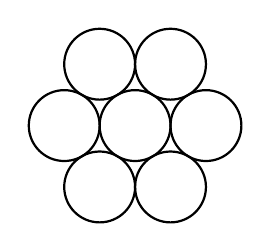
\begin{tikzpicture}[scale=0.9]
  \draw[thick] (0,0) circle (0.5);
  \foreach \k in {0,...,5} { \draw[thick] ({\k*60}:1) circle (0.5); }
\end{tikzpicture}
\end{center}

The idea of the proof was to use \emph{saturation} and the \emph{Delaunay triangulation}.

\begin{remark}
In the proof we left out the error analysis of the limits, etc.
\end{remark}

\begin{remark}
Rogers showed a density bound coming from the regular simplex.
\added{Precisely (C.~A.~Rogers, 1958): the density of any packing of unit balls in $\R^n$ is at most the
fraction of a regular simplex of edge length $2$ that is covered by the $n+1$ unit balls centred at its
vertices. For $n=2$ this is exactly $\pi/\sqrt{12}$, so Rogers' bound generalizes Thue's theorem.}
\end{remark}

% ---------------------------------------------------------------------------
\section{The Fejes T\'oth inequality for \texorpdfstring{$\Sph^2$}{S2}}\label{L2:sec:FT}

All distances on $\Sph^2$ are spherical (angular) distances.

\begin{theorem}[Fejes T\'oth\added{, 1943}]\label{L2:thm:FT}
For any $n\ge 3$ points on $\Sph^2$ there exists a pair with spherical distance
\begin{equation}\label{L2:eq:FT}
d \;\le\; \arccos\!\left(\frac{\cot^2(\omega)-1}{2}\right),
\qquad \omega=\frac{n}{n-2}\cdot\frac{\pi}{6}. \tag{$*$}
\end{equation}
\end{theorem}
\fixed{Notes have $\cot(\omega)$; must be $\cot^2(\omega)$.}

\begin{addedblock}
Check: for $n=12$, $\omega=\pi/5$, and $(\cot^2(\pi/5)-1)/2 = 1/\sqrt5$, so
$d\le\arccos(1/\sqrt5)\approx 63.43^\circ$, the edge of the regular icosahedron. Similarly $n=3,4,6$ give
$120^\circ$, $\arccos(-1/3)\approx109.47^\circ$ and $90^\circ$ (equilateral triangle on a great circle,
regular tetrahedron, regular octahedron). These are exactly the cases in which the bound is attained.
\end{addedblock}

\begin{remark}\label{L2:rem:capdensity}
The inequality can be rewritten as a density result for spherical caps of diameter $d$ (i.e.\ angular
radius $d/2$): a cap of angular radius $r$ has area $2\pi(1-\cos r)$, so the density of $n$ non-overlapping
caps of diameter $d$ is
\[
\frac{n\cdot 2\pi\bigl(1-\cos(d/2)\bigr)}{4\pi}
\added{\ \le\ \frac n2\Bigl(1-\cos\tfrac{d_n}{2}\Bigr)}
\;\longrightarrow\; \frac{\pi}{\sqrt{12}}
\added{\quad (n\to\infty),}
\]
\added{where $d_n$ is the right-hand side of \eqref{L2:eq:FT}.} So in the limit we recover Thue's bound.
\end{remark}

\begin{exercise}
Verify the limit in Remark~\ref{L2:rem:capdensity}. \added{(Hint: as $n\to\infty$, $d_n\to 0$ and
$\frac{\sqrt3}{4}d_n^2\sim \frac{4\pi}{2n}$; see also Exercise~\ref{L2:ex:Lhuilier}.)}
\end{exercise}

The ``flat'' values also converge, but it is not so nice to take the limit.
\unclear{``Flat values'': presumably the planar triangles of the convex hull instead of spherical ones.}

A natural question: is there a good \emph{lower} bound, i.e.\ can we construct a sequence of sets of
points that achieves this bound?
\begin{addedblock}
Equality in \eqref{L2:eq:FT} holds only for $n=3,4,6,12$. Asymptotically the bound is sharp: there are
configurations (e.g.\ suitable subdivisions of the icosahedron) whose cap density tends to
$\pi/\sqrt{12}$.
\end{addedblock}

\subsection{A lemma on spherical triangles}

To prove the Fejes T\'oth theorem we need the following lemma.

\begin{lemma}\label{L2:lem:triangle}
Let $ABC$ be a spherical triangle and let $\overline{AB}$ be its shortest side. Let $ABC'$ be the
equilateral spherical triangle drawn on $\overline{AB}$\added{, with $C'$ on the same side of the great
circle $AB$ as $C$}. If
\[
\operatorname{Area}(ABC) < \operatorname{Area}(ABC'),
\]
then the spherical radius of the circumcircle of $ABC$ (the circle in which the plane through $A,B,C$
meets $\Sph^2$) is greater than the length of $\overline{AB}$.
\end{lemma}

\begin{proof}
Write $a$ for the length of $\overline{AB}$.

\emph{Step 1: draw the picture.} Let $C'$ be such that $ABC'$ is equilateral, with $C'$ on the same side
of the great circle $AB$ as $C$. Let $\alpha,\beta,\gamma$ be the circles of radius $a$ centred at
$A,B,C'$ respectively\added{; thus $\alpha$ passes through $B$ and $C'$, $\beta$ through $A$ and $C'$,
and $\gamma$ through $A$ and $B$}. Let $A'$ be the second intersection point of $\alpha$ and $\gamma$
\added{(so that $AC'A'$ is equilateral)}, and $B'$ the second intersection point of $\beta$ and $\gamma$.
Let $-A,-B$ denote the antipodes of $A,B$.

\begin{figure}[ht]
\centering
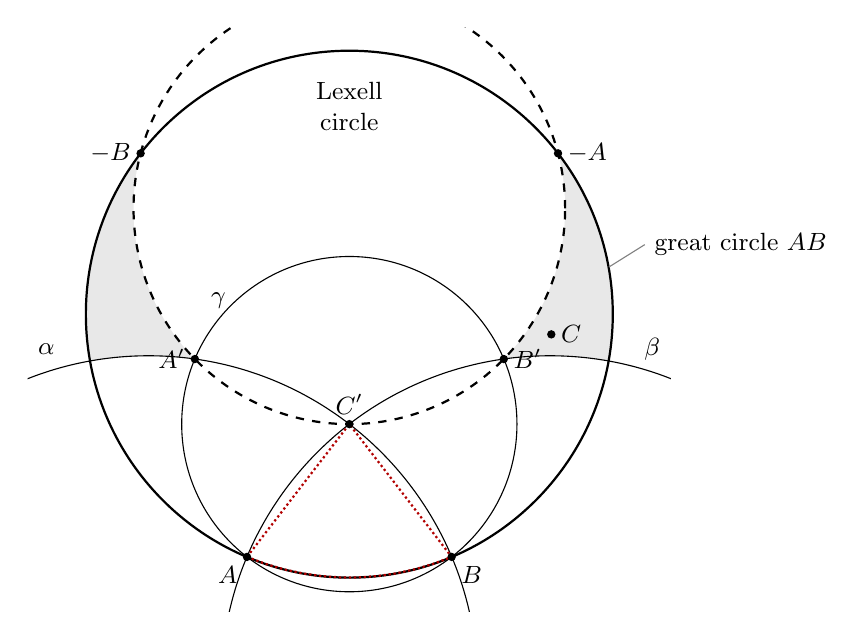
\begin{tikzpicture}[scale=0.95]
  \begin{scope}
    \clip (-4.3,-2.5) rectangle (4.3,5.3);
    % admissible region for C: C' side of AB, below the Lexell circle, outside alpha and beta
    \fill[gray!18] (0,1.470) circle (3.522);
    \fill[white] (0,2.885) circle (2.885);
    \fill[white] (-2.683,-3.482) circle (4.396);
    \fill[white] (2.683,-3.482) circle (4.396);
    % circles
    \draw[thick] (0,1.470) circle (3.522);                 % great circle AB
    \draw[thick,dashed] (0,2.885) circle (2.885);          % Lexell circle
    \draw (-2.683,-3.482) circle (4.396);                  % alpha
    \draw (2.683,-3.482) circle (4.396);                   % beta
    \draw (0,0) circle (2.241);                            % gamma
  \end{scope}
  % equilateral triangle ABC' (great-circle arcs)
  \draw[red!70!black,densely dotted,thick] (-1.368,-1.775) -- (-1.122,-1.868) -- (-0.875,-1.941) -- (-0.626,-1.995) -- (-0.376,-2.031) -- (-0.125,-2.049) -- (0.125,-2.049) -- (0.376,-2.031) -- (0.626,-1.995) -- (0.875,-1.941) -- (1.122,-1.868) -- (1.368,-1.775)
     -- (1.212,-1.573) -- (1.067,-1.384) -- (0.930,-1.207) -- (0.800,-1.038) -- (0.676,-0.877) -- (0.557,-0.722) -- (0.441,-0.572) -- (0.328,-0.426) -- (0.218,-0.283) -- (0.109,-0.141) -- (0,0)
     -- (-0.109,-0.141) -- (-0.218,-0.283) -- (-0.328,-0.426) -- (-0.441,-0.572) -- (-0.557,-0.722) -- (-0.676,-0.877) -- (-0.800,-1.038) -- (-0.930,-1.207) -- (-1.067,-1.384) -- (-1.212,-1.573) -- cycle;
  % points
  \foreach \p/\n/\pos in {(-1.368,-1.775)/A/below left, (1.368,-1.775)/B/below right, (0,0)/C'/above,
      (-2.065,0.870)/A'/left, (2.065,0.870)/B'/right, (2.790,3.620)/-A/right, (-2.790,3.620)/-B/left}
      { \fill \p circle (1.6pt) node[\pos,font=\small] {$\n$}; }
  \fill (2.7,1.2) circle (1.6pt) node[right,font=\small] {$C$};
  % labels
  \node[font=\small] at (-4.05,1.0) {$\alpha$};
  \node[font=\small] at (4.05,1.0) {$\beta$};
  \node[font=\small] at (-1.75,1.65) {$\gamma$};
  \node[font=\small,align=center] at (0,4.25) {Lexell\\circle};
  \draw[thin,gray] (3.47,2.1) -- (3.95,2.4) node[right,font=\small,black] {great circle $AB$};
\end{tikzpicture}
\caption{The configuration of Lemma~\ref{L2:lem:triangle} (side $a=70^\circ$), drawn in stereographic
projection centred at $C'$, so circles on $\Sph^2$ appear as circles. Shaded: the points between the great circle $AB$ and the Lexell circle that lie outside $\alpha$ and
$\beta$ (the possible positions of $C$); they avoid the disc bounded by $\gamma$.}
\label{L2:fig:lexell}
\end{figure}
\orig{Hand sketch p.~19 has the great circle $AB$ as a straight line; redrawn exactly here.}

\emph{Step 2: show the picture is ``correct''.} Note that the spherical triangles $ABA'$, $ABB'$ and $ABC'$
all have equal area. \added{(For $ABA'$: it is isosceles with legs $a$ and apex angle $2\theta$, where
$\theta$ is the angle of $ABC'$; a direct computation with the formula
$\tan\frac E2=\frac{\sin\varphi\,\tan\frac b2\tan\frac c2}{1+\cos\varphi\,\tan\frac b2\tan\frac c2}$ for the
area $E$ of a triangle with sides $b,c$ and included angle $\varphi$, together with
$\tan^2\frac a2=1-2\cos\theta$, shows that both areas agree.)} Hence the circle in which the plane through
$\{A',B',C'\}$ meets the sphere is the locus of points $X$ with
$\operatorname{Area}(ABX)=\operatorname{Area}(ABC')$ (on that side of $AB$): this is the
\emph{Lexell circle theorem}. \added{(Lexell: for fixed $A,B$, the locus of apexes $X$ of triangles $ABX$
of fixed area is an arc of a small circle through $-A$ and $-B$.)}

By assumption, $\operatorname{Area}(ABC)<\operatorname{Area}(ABC')$, so $C$ lies between the Lexell circle
and the great circle $AB$. As $\overline{AB}$ is the shortest edge of $ABC$, $C$ does not lie in
\added{the open discs bounded by} $\alpha$ or $\beta$. It follows \added{(see
Figure~\ref{L2:fig:lexell})} that $C$ does not lie in \added{the disc bounded by} $\gamma$.
\added{(The part of the disc of $\gamma$ on the $C'$ side of $AB$ and below the Lexell circle is covered by
the discs of $\alpha$ and $\beta$.)}
\unclear{This covering step is read off the picture in the notes.}

But $C$ is on the $C'$ side of $AB$. \added{The circles through $A$ and $B$ form a pencil whose centres lie
on the perpendicular bisector of $AB$; on the $C'$ side, the region enclosed by such a circle grows with its
radius. Since $\gamma$ is the member of the pencil centred at $C'$ and $C$ lies outside it,} the
circumcircle of $ABC$ has radius greater than the radius of $\gamma$, which is the length of
$\overline{AB}$.
\end{proof}

\subsection{Proof of the Fejes T\'oth theorem}

The case $n=3$ is trivial\added{: the three sides of a spherical triangle have total length at most
$2\pi$, so one of them is at most $2\pi/3=\arccos(-1/2)$}. So let $n\ge 4$ and let $p_1,\dots,p_n\in\Sph^2$.

Without loss of generality the convex hull $\conv\{p_1,\dots,p_n\}$ contains the origin $0$
\added{in its interior}. Otherwise we could flow the points from the pole towards the equator
\added{of a hemisphere containing them} and increase all distances.
\begin{addedblock}
If all points lie in an open hemisphere with pole $N$, replace the colatitude $\phi$ (angle from $N$) of
each point by $\lambda\phi$, $\lambda>1$ close to $1$. From
$\cos d=\cos\phi_1\cos\phi_2+\sin\phi_1\sin\phi_2\cos\Delta$ one checks
$\frac{\partial}{\partial\lambda}\cos d\le-(\phi_1-\phi_2)\sin(\phi_1-\phi_2)\le0$, with strict
inequality for distinct points, so all mutual distances increase.
\end{addedblock}
\unclear{Degenerate case (points in a closed, not open, hemisphere) needs a small perturbation argument.}

\emph{Step 1: triangulate the convex hull.}
\added{The convex hull is a polytope whose vertices are among the $p_i$; after a small perturbation (which
changes distances only slightly) we may assume it is simplicial, with all $n$ points as vertices.}
By the Euler characteristic, it has $2n-4$ faces.

\begin{exercise}\label{L2:ex:euler}
Show that a triangulated convex polytope with $n$ vertices has $2n-4$ faces.
\emph{Solution sketch:} $v-e+f=2$ and $3f=2e$ for triangulations; hence $2n-2e+2f=4$, so
$2n-3f+2f=4$, i.e.\ $f=2n-4$.
\end{exercise}

The triangulation of $\conv\{p_1,\dots,p_n\}$ gives a \emph{spherical net} by radial projection to the
sphere: the edges become geodesic arcs\added{, and since $0$ is in the interior of the hull the $2n-4$
spherical triangles tile $\Sph^2$}.

\begin{center}
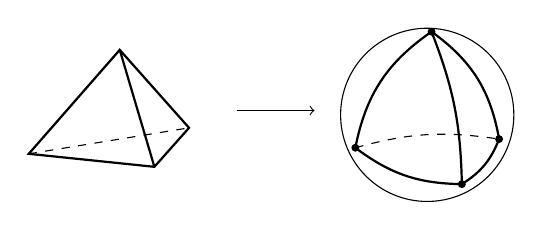
\begin{tikzpicture}[scale=1.1]
  % tetrahedron
  \coordinate (P1) at (-1.0,-0.45); \coordinate (P2) at (0.45,-0.6);
  \coordinate (P3) at (0.85,-0.15); \coordinate (P4) at (0.05,0.75);
  \draw[thick] (P1)--(P2)--(P3)--(P4)--cycle (P4)--(P2);
  \draw[dashed] (P1)--(P3);
  \draw[->] (1.4,0.05) -- (2.3,0.05);
  % spherical net
  \begin{scope}[xshift=3.6cm]
    \draw (0,0) circle (1);
    \draw[thick] (-0.83,-0.38) to[bend right=18] (0.40,-0.80);
    \draw[thick] (0.40,-0.80) to[bend right=18] (0.83,-0.28);
    \draw[thick] (0.83,-0.28) to[bend right=22] (0.05,0.96);
    \draw[thick] (0.05,0.96) to[bend right=22] (-0.83,-0.38);
    \draw[thick] (0.05,0.96) to[bend left=10] (0.40,-0.80);
    \draw[dashed] (-0.83,-0.38) to[bend left=12] (0.83,-0.28);
    \foreach \p in {(-0.83,-0.38),(0.40,-0.80),(0.83,-0.28),(0.05,0.96)} \fill \p circle (1.3pt);
  \end{scope}
\end{tikzpicture}
\end{center}

\emph{Step 2.} Now, for $\{p_1,\dots,p_n\}$, suppose that
\[
\operatorname{length}\bigl(\widehat{p_ip_j}\bigr) > d \qquad\text{for all } i\ne j,
\]
where $d=d_n$ is the right-hand side of \eqref{L2:eq:FT}.

\begin{exercise}[L'Huilier]\label{L2:ex:Lhuilier}
Show that $d$ in \eqref{L2:eq:FT} is the side length of an equilateral spherical triangle of area
$\dfrac{4\pi}{2n-4}$. \added{(One can use L'Huilier's formula, the spherical analogue of Heron's formula.
Alternatively: the angle $\theta$ of such a triangle satisfies $3\theta-\pi=\frac{2\pi}{n-2}$, i.e.\
$\theta=2\omega$, and the spherical law of cosines for angles gives
$\cos d=\frac{\cos\theta}{1-\cos\theta}=\frac{\cot^2\omega-1}{2}$.)}
\end{exercise}

Then the triangle $p_ip_jp_k$ of minimal area in the spherical net satisfies the hypotheses of the Lemma:
its area is small, but its edges are all longer than $d$. Here ``small'' means: less than or equal to
the area of the equilateral triangle of side length $d$\added{, since $2n-4$ triangles of total area $4\pi$
tile the sphere. As the area of an equilateral triangle increases with its side, and the shortest side of
$p_ip_jp_k$ is longer than $d$, the hypothesis of Lemma~\ref{L2:lem:triangle} holds with strict
inequality.}

Hence the circumcircle of $p_ip_jp_k$ has radius larger than $d$. But the net construction implies that
the circumcircle is empty\added{: the face $p_ip_jp_k$ lies in a supporting plane of the convex hull, so no
$p_l$ lies in the open cap cut off by that plane (and this cap is smaller than a hemisphere, since $0$ is on
the other side)}.

So we may place a new point at the centre \added{of this cap; it has distance greater than $d$ from every
$p_l$}. This new collection of $n+1$ points satisfies the same inequalities for the \emph{same}~$d$!
\added{Moreover the new hull still contains $0$ in its interior and has $2(n+1)-4$ faces, so its smallest
triangle again has area less than that of the equilateral triangle of side $d$, and we can repeat
indefinitely.}

This is absurd, e.g.\ by a volume bound: $\vol(\Sph^2)=4\pi$, and \added{the caps of radius $d/2$ around the
points are pairwise disjoint, so} we would have
\[
\sum_{i=1}^{N}\operatorname{area}\bigl(\operatorname{cap}(d/2)\bigr) < 4\pi \qquad\text{for all } N>0,
\]
\added{which is impossible since each cap has positive area.} \qed

% ---------------------------------------------------------------------------
\section{Higher-dimensional sphere packing: Blichfeldt's method}\label{L2:sec:blichfeldt}

Consider an early method of Blichfeldt (1929) to get density bounds in higher dimensions.
\added{(H.~F.~Blichfeldt, \emph{The minimum value of quadratic forms, and the closest packing of spheres},
Math.\ Ann.\ 101 (1929).)}

\begin{definition}\label{L2:def:convexbody}
A \emph{convex body} $C$ in $\R^n$ is a compact convex subset of $\R^n$ with non-empty interior.
\end{definition}
\orig{Crossed out: ``(so think $C=\mathbb{B}^n$)''.}

Also consider collections of isometries $\{\varphi_i\}_{i=1}^\infty$ of $\R^n$ such that
$\{\varphi_iC\}_{i=1}^\infty$ is a packing \added{(i.e.\ the interiors of the $\varphi_iC$ are pairwise
disjoint)}.

For now, $C=\Ball^n$ \added{is the closed unit ball}, and a packing is of the form
$\{\varphi_i\Ball^n\}_{i=1}^\infty$.

Consider replacing the ball with its characteristic function
\[
\chi(x)=\begin{cases}1, & |x|\le1,\\ 0, & |x|>1.\end{cases}
\]
So it has mass
\[
I(\chi)=\int_{\R^n}\chi(x)\,dx \;\added{=\vol(\Ball^n)},
\]
and a packing corresponds to the function
\[
x\longmapsto\sum_{i=1}^\infty\chi(\varphi_i^{-1}x)
\]
\added{(the characteristic function of $\bigcup_i\varphi_i\Ball^n$, up to the measure-zero set of boundary
points).} For a general convex body $C$ this works as well.

Furthermore, we can now replace $\chi$ with some other function $f$, and in general associate to a packing
the function
\[
x\longmapsto\sum_{i=1}^\infty f(\varphi_i^{-1}x).
\]
A density may be defined similarly to the packing density, where each object now has mass
\[
I(f)=\int_{\R^n}f(x)\,dx
\]
spread over $\operatorname{supp}(f)$. So:
\[
\Delta_f \;=\; \dens_{\text{packing}}\cdot\frac{I(f)}{\vol(C)}.
\]
\added{Here $\dens_{\text{packing}}$ is the density of the packing $\{\varphi_iC\}$ (Lecture~1), i.e.\ the
average number of copies per unit volume times $\vol(C)$; $\Delta_f$ is the average of
$\sum_i f(\varphi_i^{-1}x)$ over $x\in\R^n$.}

We can think of this as spreading out and renormalizing the characteristic function in some (nice,
hopefully) way: ``cut up the sphere and spread it out.''

\textbf{Insight.} There are functions $f$ for which the sums $\sum_{i=1}^\infty f(\varphi_i^{-1}x)$ are
uniformly pointwise bounded over $\R^n$ \emph{and} over all collections of isometries $\{\varphi_i\}$ such
that $\{\varphi_iC\}$ is a packing!

% ---------------------------------------------------------------------------
\section{Blichfeldt gauges}\label{L2:sec:gauge}

\begin{definition}\label{L2:def:gauge}
Given a convex body $C$ in $\R^n$, a \added{non-negative, integrable} function $f$ on $\R^n$ is a
\emph{Blichfeldt gauge} for $C$ if for any collection $\{\varphi_i\}_{i=1}^\infty$ of isometries of
$\R^n$ such that $\{\varphi_iC\}_{i=1}^\infty$ is a packing,
\[
\sum_{i=1}^\infty f(\varphi_i^{-1}x)\le 1 \qquad\text{for all } x\in\R^n.
\]
\end{definition}
\fixed{Notes: ``isometries of $\R^d$''; should be $\R^n$.}
\orig{Margin: ``add non-negative condition''.}

\begin{lemma}\label{L2:lem:gauge}
If $f$ is a Blichfeldt gauge for $C$, then the density of any packing of $\R^n$ by copies of $C$ satisfies
\[
\dens(C)\;\le\;\frac{\vol(C)}{I(f)}. \tag{$**$}
\]
\end{lemma}
\fixed{Notes have strict $<$; equality can occur (e.g.\ $f=\chi_{\interior C}$, $C$ a cube).}

\begin{proof}[Proof sketch]
By the definition, $\Delta_f\le 1$ \added{(the average of a function bounded by $1$ is at most $1$)}.
Since $\Delta_f=\dens\cdot I(f)/\vol(C)$, this gives $(**)$. \added{The limiting argument that makes this
precise is carried out for balls in Section~\ref{L2:sec:bound}; the same argument works for any $C$ and any
gauge with bounded support.}
\end{proof}

% ---------------------------------------------------------------------------
\section{Back to \texorpdfstring{$C=\Ball^n$}{C = B\^{}n}}\label{L2:sec:radial}

We can consider radially symmetric functions by an averaging argument: there is no benefit to anisotropy,
since $\SO(n)$ kills it.
\begin{addedblock}
If $f$ is a gauge for $\Ball^n$, so is $\bar f(x)=\int_{\SO(n)}f(gx)\,dg$ (Haar probability measure):
for each $g$, $\{\varphi_ig^{-1}\Ball^n\}=\{\varphi_i\Ball^n\}$ is the same packing, so
$\sum_i f(g\varphi_i^{-1}x)\le1$, and averaging over $g$ gives $\sum_i\bar f(\varphi_i^{-1}x)\le 1$.
Moreover $I(\bar f)=I(f)$, so $\bar f$ gives the same bound.
\end{addedblock}
So it suffices to consider functions of the distance $|x|$! Rankin does a complicated study to get a good
function \added{(R.~A.~Rankin, \emph{On the closest packing of spheres in $n$ dimensions}, Ann.\ of Math.\
48 (1947))}. We consider
\[
f_0(x)=\begin{cases}1-\tfrac12|x|^2, & |x|\le\sqrt2,\\[2pt] 0, & |x|>\sqrt2.\end{cases}
\]

We can show the following for a packing of unit radius balls.

\begin{lemma}\label{L2:lem:f0}
$f_0$ is a Blichfeldt gauge for $\Ball^n$.
\end{lemma}

\begin{proof}
Consider $m$ unit balls \added{in a packing} with centres $x_1,\dots,x_m\in\R^n$. Then clearly, for all
pairs,
\[
|x_i-x_j|^2\ge 4. \tag{$\dagger$}
\]
Summing $(\dagger)$ over $1\le i<j\le m$ (the cross terms cancel\added{, via the identity
$\sum_{i<j}|x_i-x_j|^2=m\sum_i|x_i|^2-\bigl|\sum_ix_i\bigr|^2$}), we get
\[
m\sum_{i=1}^m|x_i|^2-\Bigl|\sum_{i=1}^m x_i\Bigr|^2\;\ge\;2m(m-1),
\]
and therefore
\[
\sum_{i=1}^m|x_i|^2\;\ge\;2(m-1).
\]
\orig{Notes write the centres in coordinates $(a_i,b_i,\dots,n_i)$.}
The origin here is an arbitrary point. So, given $x\in\R^n$, consider the collection of the $m$ balls whose
centres lie within $\sqrt2$ of $x$ \added{(the only ones contributing to $\sum_if_0(x-x_i)$)}, with masses
defined by $f_0$ centred at the $x_i$. Writing $r_i=|x-x_i|$, we see that
\[
\sum_{i=1}^m\frac{2-r_i^2}{2}\;\le\;\frac{2m-2(m-1)}{2}\;=\;1,
\]
and so $f_0$ is a Blichfeldt gauge.
\end{proof}

% ---------------------------------------------------------------------------
\section{Blichfeldt's bound}\label{L2:sec:bound}

So we can integrate this, using spherical shells:
\[
I(f_0)=\int_0^{\sqrt2}\frac{2-r^2}{2}\,d\bigl(\vol(\Ball^n)\,r^n\bigr)
=\frac{2^{\frac n2+1}}{n+2}\,\vol(\Ball^n).
\]
\fixed{Notes first had $\frac{4\cdot2^{n/2}}{n+2}$; corrected in red to $\frac{2^{(n+2)/2}}{n+2}$.}

\begin{exercise}\label{L2:ex:integral}
Verify this integral using spherical shells. \added{($I(f_0)=n\vol(\Ball^n)\int_0^{\sqrt2}
(1-\tfrac{r^2}{2})r^{n-1}dr=\vol(\Ball^n)\,2^{n/2}\bigl(1-\tfrac{n}{n+2}\bigr)$.)}
\end{exercise}

\subsection*{Limit argument for a box}

Take a large box of side length $t$ with $K$ balls in it.
\orig{Notes write $|I|$ for $K$.}
\added{Their centres lie in the concentric box of side $t-2$, so the supports of the gauges
$f_0(x-x_i)$ lie in the concentric box of side} $t+2\sqrt2-2$. Since $f_0\ge 0$ and
$\sum_if_0(x-x_i)\le1$ everywhere, integrating over this larger box gives
\[
(t+2\sqrt2-2)^n\;\ge\;K\int_{\R^n}f_0(x)\,dx\;=\;\frac{K\,\vol(\Ball^n)\,2^{\frac n2+1}}{n+2}.
\]
Hence the density of these $K$ balls in the box $[0,t]^n$ satisfies
\[
\frac{K\vol(\Ball^n)}{t^n}\;\le\;\frac{n+2}{2^{\frac n2+1}}\Bigl(1+\frac{2\sqrt2-2}{t}\Bigr)^n,
\]
and letting $t\to\infty$:

\begin{theorem}[Blichfeldt's bound]\label{L2:thm:blichfeldt}
For any packing of $\R^n$ by unit balls,
\[
\dens\;\le\;\frac{n+2}{2^{\frac n2+1}} \;=\; \frac{n+2}{2}\,2^{-n/2}.
\]
\end{theorem}
\fixed{Notes had $\frac{n+2}{4\cdot2^{n/2}}$ (red correction in margin).}

One can do this explicitly for balls too; we are also still missing a boundary term.
\unclear{Probably: balls meeting the boundary of the box; they contribute $O(t^{n-1})$, negligible as $t\to\infty$.}

\begin{remark}
\added{For $n=2$ the bound is the trivial $\dens\le1$; for $n=3$ it gives $5/(4\sqrt2)\approx0.884$, compared
with $\pi/\sqrt{18}\approx0.7405$ for the FCC packing (Rogers' simplex bound gives $\approx0.7797$).
Blichfeldt's bound decays like $2^{-0.5n}$ up to polynomial factors; Rankin (1947) improved the constant,
and Kabatiansky--Levenshtein (1978) improved the exponent to $2^{-0.599n}$.}
\end{remark}
